% Copyright 2007 by Till Tantau
%
% This file may be distributed and/or modified
%
% 1. under the LaTeX Project Public License and/or
% 2. under the GNU Public License.
%
% See the file doc/licenses/LICENSE for more details.

\documentclass[10pt]{beamer}
\usepackage[normalem]{ulem}
\renewcommand{\AA}{\mathbb{A}}
\newcommand{\BB}{\mathbb{B}}

\newcommand{\RR}{\mathbb{R}}
\newcommand{\CC}{\mathbb{C}}
\newcommand{\LL}{\mathbb{L}}
\newcommand{\MM}{\mathbb{M}}
\newcommand{\ZZ}{\mathbb{Z}}
\newcommand{\QQ}{\mathbb{Q}}
\newcommand{\LLp}{\LL}
\newcommand{\conj}[1]{{\bar{#1}}}
\newcommand{\Arg}[1]{{\mathrm{Arg}~{#1} }}
\newcommand{\vect}{{\operatorname {vec}~}}
\newcommand{\acos}{{\operatorname {acos}}}
\newcommand{\atan}{{\operatorname {atan}}}
\newcommand{\dist}{{\operatorname {dist}}}
\newcommand{\argmin}{{\operatorname {argmin}}}

\newcommand{\kron}{\otimes}
\newtheorem{prob}[theorem]{Problem}
\newcommand{\diag}{\operatorname{diag}}
\newcommand{\re}{\operatorname{Re}}
\newcommand{\im}{\operatorname{Im}}

\newcommand{\mycite}[1]{$[$#1$]$}
\newcount\mytildegroup
 \newcommand\undertildetweak{\mathpalette\undertildeint}
 \def\undertildeint#1#2{%
   \oalign{%
      $\mathgroup\mytildegroup#1#2$%
     \crcr
      \hidewidth
      \vbox to.5ex{% 
        \hbox{%
          $\hss
           #1%
              \widetilde{~~}
 %          \widetilde{\hspace{20pt}}%  % If the tilde is not wide enough
           \hss$}%
        \vss}%
      \hidewidth}}
 \newcommand{\subseteqsim}{\undertildetweak{\subseteq}}
 \newcommand{\subsetsim}{\undertildetweak{\subset}}


%\input{pres-style-new.tex}
\newcommand{\DD}{\mathbb{D}}
%\newcommand{\BB}{\mathbb{B}}
\newcommand{\BBB}{\mathcal{B}}
\newcommand{\CalD}{\mathcal{D}}

\newcommand{\htwonorm}[1]{\|#1\|_2} 
%\newcommand{\htwonorm}[1]{\|#1\|_{H_2}} 
\newcommand{\htwo}{${\cal H}_2${}} 
\newcommand{\tr}{\operatorname{Tr}}
\newcommand{\veps}{\varepsilon}

%\usepackage{fancybox}
%\usepackage{lmodern}

%%%%%%%% tikz/pgf stuff: 
\newcommand{\defaultmarksize}{3pt}
\usepackage{tikz,pgfplots}
\usepackage{pgf}
%\usepackage{pgfmath}
\usepackage{pgffor}
%\pgfrealjobname{aof}
\usetikzlibrary{matrix}
\usetikzlibrary{calc}
\usetikzlibrary{arrows}
\usetikzlibrary{decorations.markings}
\usetikzlibrary{shapes,snakes}
\usetikzlibrary{calc}
\usetikzlibrary{plotmarks}
\usetikzlibrary{patterns}
\usepgflibrary[shapes.geometric]
\usetikzlibrary{snakes}
\usetikzlibrary{shapes.geometric}
\pgfplotsset{compat=newest}
%\pgfplotsset{plot coordinates/math parser=false}
\usepgflibrary{plothandlers}    
%
\newlength\figurewidth 
%\newcommand{\myinputfigg}[1]{\beginpgfgraphicnamed{gfx/#1}\setlength\figurewidth{0.5\textwidth}
%\input{gfx/#1.tikz}\endpgfgraphicnamed}
\newcommand{\myinputfigg}[1]{\setlength\figurewidth{0.8\textwidth}\input{gfx/#1.tikz}}
%%\newcommand{\myinputfigg}[1]{\setlength\figurewidth{1.0\textwidth}
%%\input{gfx/#1.tikz}}

%\newcommand{\myinputfiggsmall}[1]{\beginpgfgraphicnamed{gfx/#1}\setlength\figurewidth{0.48\textwidth}
%\input{gfx/#1.tikz}\endpgfgraphicnamed}
%%\newcommand{\myinputfiggsmall}[1]{\setlength\figurewidth{0.48\textwidth}
%%\input{gfx/#1.tikz}}
%\pgfplotsset{plot coordinates/math parser=false} 
%\pgfplotsset{compat=newest}
%


\begin{document}
%%
\begin{frame}
  \maketitle
\end{frame}
\begin{frame}

{\bf Presentation outline:}\\~\\
Part 1. WEP: Waveguide eigenvalue problem\\
Part 2. TIAR: Tensor infinite Arnoldi method\\
Part 3. Specialization of TIAR to WEP\\
Part 4. Numerical simulations
\end{frame}
\section{WEP}
\begin{frame}
\begin{center}
\Large
\bf 1. Waveguide eigenvalue problem (WEP)\\\vspace{0.5cm}
%\bf Thanks to COMSOL and KTH for DqF-financing!
%\vspace{2cm}
\end{center}
\end{frame}
\begin{frame}
\begin{block}{Helmholtz equation (single-periodic coefficients):}\vspace{-0.8cm}
\begin{eqnarray*}
  \Delta u(x,z)+\kappa(x,z)^2u(x,z)&=&0\;\; \textrm{when }\; (x,z)\in\RR\times\RR\\
  u(x,\cdot)&\rightarrow& 0\;\;\textrm{as }\; x\rightarrow\pm\infty
\end{eqnarray*}\vspace{-0.6cm}
\begin{itemize}
  \item $\kappa(x,z)$ periodic $z$-direction. 
  \item $\kappa(x,z)$ constant for $(x,z)\not\in[x_-,x_+]\times\RR$. 
\end{itemize}\vspace{-0.2cm}
\end{block}
\begin{overlayarea}{\textwidth}{4cm}\begin{center}
\only<2>{\scalebox{0.8}{%\tikzsetnextfilename{waveguidefig2} % name for the temporary 
\definecolor{cbebebf}{RGB}{200,200,200}%
\begin{tikzpicture}[remember picture, y=0.80pt,x=0.80pt,yscale=-0.25,xscale=0.25, inner sep=0pt, outer sep=0pt]
  %\path [use as bounding box,red] (300,112) rectangle (20.0000,292.36);
  \path[fill=cbebebf,line join=miter,line cap=butt,even odd rule,line
    width=0.800pt,rounded corners=0.0000cm] (70.0000,112.3622) rectangle
    (680.0000,292.3622);
  \node at (360,60) {$\vdots$};
  \node at (0.0000,180) (myref) {};
%  \path[draw=black,line join=miter,line cap=butt,line width=0.800pt]
%    (650.0000,112.3622) .. controls (100.0000,112.3622) and (100.0000,112.3622) ..
%    (100.0000,112.3622);
%  \path[draw=black,line join=miter,line cap=butt,line width=0.800pt]
%    (650.5000,291.8622) .. controls (100.5000,291.8622) and (100.5000,291.8622) ..
%    (100.5000,291.8622);
  \path[draw=black,line join=miter,line cap=butt,line width=1.800pt]
    (300.0000,112.3622) -- (300.0000,292.3622) -- (300.0000,292.3622);
  \path[draw=black,line join=miter,line cap=butt,line width=1.800pt]
    (380.0000,112.3622) -- (380.0000,232.3622) -- (420.0000,232.3622) --
    (420.0000,292.3622) -- (420.0000,292.3622);
  \path[fill=black] (255.56859,334.04221) node (text3878) {\phantom{$\;\;\;\partial\Omega_-$}};
  \path[fill=black] (440.42651,334.04221) node[right] (text3882) {\phantom{$\partial\Omega_+$   }};
  \node at (0,690) {};
\end{tikzpicture}%
\begin{tikzpicture}[remember picture, y=0.80pt,x=0.80pt,yscale=-0.25,overlay, shift={(myref.north)}, xscale=0.25, inner sep=0pt, outer sep=0pt]
  \path[fill=cbebebf,line join=miter,line cap=butt,even odd rule,line
    width=0.800pt,rounded corners=0.0000cm] (70.0000,112.3622) rectangle
    (680.0000,292.3622);
  \node at (0.0000,180) (myref2) {};
%  \path[draw=black,line join=miter,line cap=butt,line width=0.800pt]
%    (650.0000,112.3622) .. controls (100.0000,112.3622) and (100.0000,112.3622) ..
%    (100.0000,112.3622);
%  \path[draw=black,line join=miter,line cap=butt,line width=0.800pt]
%    (650.5000,291.8622) .. controls (100.5000,291.8622) and (100.5000,291.8622) ..
%    (100.5000,291.8622);
  \path[draw=black,line join=miter,line cap=butt,line width=1.800pt]
   (300.0000,112.3622) -- (300.0000,292.3622) -- (300.0000,292.3622);
  \path[draw=black,line join=miter,line cap=butt,line width=1.800pt]
    (425,112.3622) --  (380.0000,112.3622) -- (380.0000,232.3622) -- (420.0000,232.3622) --
    (420.0000,292.3622) -- (420.0000,292.3622);
\end{tikzpicture}%
\begin{tikzpicture}[remember picture, y=0.80pt,x=0.80pt,yscale=-0.25,overlay, shift={(myref2.north)}, xscale=0.25, inner sep=0pt, outer sep=0pt]
  \path[fill=cbebebf,line join=miter,line cap=butt,even odd rule,line
    width=0.800pt,rounded corners=0.0000cm] (70.0000,112.3622) rectangle
    (680.0000,292.3622);
  \node at (0.0000,180) (myref3) {};
%  \path[draw=black,line join=miter,line cap=butt,line width=0.800pt]
%    (650.0000,112.3622) .. controls (100.0000,112.3622) and (100.0000,112.3622) ..
%    (100.0000,112.3622);
%  \path[draw=black,line join=miter,line cap=butt,line width=0.800pt]
%    (650.5000,291.8622) .. controls (100.5000,291.8622) and (100.5000,291.8622) ..
%    (100.5000,291.8622);
  \path[draw=black,line join=miter,line cap=butt,line width=1.800pt]
   (300.0000,112.3622) -- (300.0000,292.3622) -- (300.0000,292.3622);
  \path[draw=black,line join=miter,line cap=butt,line width=1.800pt]
    (425,112.3622) --  (380.0000,112.3622) -- (380.0000,232.3622) -- (420.0000,232.3622) --
    (420.0000,292.3622) -- (420.0000,292.3622);
  \path[<->,draw=black,line width=1pt]
    (100.0000,150) -- node[midway,left] {$z$\;\;} (100.0000,240) -- node[midway,below]{$\phantom{\Sigma^\Sigma}x\phantom{\Sigma^\Sigma}$} (200,240);
  \node at (360,320) {$\vdots$};
\end{tikzpicture}%
}}%
\only<3->{~\\~~\scalebox{0.5}{\includegraphics{schematic_full.pdf}}}
\end{center}
\end{overlayarea}
%\scalebox{0.68}{\phantom{aaaaaaaaa}\includegraphics{schematic_interior.pdf}\phantom{aaaaaaaaa}}
%
%\begin{figure}[t]
%%\begin{centering}
%%\includegraphics{gp/convergence_diagram.pdf}\;\;\;\;%
%%\includegraphics{gp/ground_state.pdf}
%%\begin{figure}
%%\begin{minipage}{1.0\paperwidth}
%\begin{center}
%\subfigure[Illustration of the waveguide.
%The wave number $\kappa(x,z)$  is constant in the three 
%regions separated by the
%thick lines. 
%]{%\tikzsetnextfilename{waveguidefig2} % name for the temporary 
\definecolor{cbebebf}{RGB}{200,200,200}%
\begin{tikzpicture}[remember picture, y=0.80pt,x=0.80pt,yscale=-0.25,xscale=0.25, inner sep=0pt, outer sep=0pt]
  %\path [use as bounding box,red] (300,112) rectangle (20.0000,292.36);
  \path[fill=cbebebf,line join=miter,line cap=butt,even odd rule,line
    width=0.800pt,rounded corners=0.0000cm] (70.0000,112.3622) rectangle
    (680.0000,292.3622);
  \node at (360,60) {$\vdots$};
  \node at (0.0000,180) (myref) {};
%  \path[draw=black,line join=miter,line cap=butt,line width=0.800pt]
%    (650.0000,112.3622) .. controls (100.0000,112.3622) and (100.0000,112.3622) ..
%    (100.0000,112.3622);
%  \path[draw=black,line join=miter,line cap=butt,line width=0.800pt]
%    (650.5000,291.8622) .. controls (100.5000,291.8622) and (100.5000,291.8622) ..
%    (100.5000,291.8622);
  \path[draw=black,line join=miter,line cap=butt,line width=1.800pt]
    (300.0000,112.3622) -- (300.0000,292.3622) -- (300.0000,292.3622);
  \path[draw=black,line join=miter,line cap=butt,line width=1.800pt]
    (380.0000,112.3622) -- (380.0000,232.3622) -- (420.0000,232.3622) --
    (420.0000,292.3622) -- (420.0000,292.3622);
  \path[fill=black] (255.56859,334.04221) node (text3878) {\phantom{$\;\;\;\partial\Omega_-$}};
  \path[fill=black] (440.42651,334.04221) node[right] (text3882) {\phantom{$\partial\Omega_+$   }};
  \node at (0,690) {};
\end{tikzpicture}%
\begin{tikzpicture}[remember picture, y=0.80pt,x=0.80pt,yscale=-0.25,overlay, shift={(myref.north)}, xscale=0.25, inner sep=0pt, outer sep=0pt]
  \path[fill=cbebebf,line join=miter,line cap=butt,even odd rule,line
    width=0.800pt,rounded corners=0.0000cm] (70.0000,112.3622) rectangle
    (680.0000,292.3622);
  \node at (0.0000,180) (myref2) {};
%  \path[draw=black,line join=miter,line cap=butt,line width=0.800pt]
%    (650.0000,112.3622) .. controls (100.0000,112.3622) and (100.0000,112.3622) ..
%    (100.0000,112.3622);
%  \path[draw=black,line join=miter,line cap=butt,line width=0.800pt]
%    (650.5000,291.8622) .. controls (100.5000,291.8622) and (100.5000,291.8622) ..
%    (100.5000,291.8622);
  \path[draw=black,line join=miter,line cap=butt,line width=1.800pt]
   (300.0000,112.3622) -- (300.0000,292.3622) -- (300.0000,292.3622);
  \path[draw=black,line join=miter,line cap=butt,line width=1.800pt]
    (425,112.3622) --  (380.0000,112.3622) -- (380.0000,232.3622) -- (420.0000,232.3622) --
    (420.0000,292.3622) -- (420.0000,292.3622);
\end{tikzpicture}%
\begin{tikzpicture}[remember picture, y=0.80pt,x=0.80pt,yscale=-0.25,overlay, shift={(myref2.north)}, xscale=0.25, inner sep=0pt, outer sep=0pt]
  \path[fill=cbebebf,line join=miter,line cap=butt,even odd rule,line
    width=0.800pt,rounded corners=0.0000cm] (70.0000,112.3622) rectangle
    (680.0000,292.3622);
  \node at (0.0000,180) (myref3) {};
%  \path[draw=black,line join=miter,line cap=butt,line width=0.800pt]
%    (650.0000,112.3622) .. controls (100.0000,112.3622) and (100.0000,112.3622) ..
%    (100.0000,112.3622);
%  \path[draw=black,line join=miter,line cap=butt,line width=0.800pt]
%    (650.5000,291.8622) .. controls (100.5000,291.8622) and (100.5000,291.8622) ..
%    (100.5000,291.8622);
  \path[draw=black,line join=miter,line cap=butt,line width=1.800pt]
   (300.0000,112.3622) -- (300.0000,292.3622) -- (300.0000,292.3622);
  \path[draw=black,line join=miter,line cap=butt,line width=1.800pt]
    (425,112.3622) --  (380.0000,112.3622) -- (380.0000,232.3622) -- (420.0000,232.3622) --
    (420.0000,292.3622) -- (420.0000,292.3622);
  \path[<->,draw=black,line width=1pt]
    (100.0000,150) -- node[midway,left] {$z$\;\;} (100.0000,240) -- node[midway,below]{$\phantom{\Sigma^\Sigma}x\phantom{\Sigma^\Sigma}$} (200,240);
  \node at (360,320) {$\vdots$};
\end{tikzpicture}%
}}\;\;%
%\begin{minipage}{0.3\textwidth}
%\vspace{-3cm}\subfigure[Floquet's theorem 
% leads to a periodic PDE \eqref{eq:helmholtz0} on a strip.
%%Artificial boundary condtions 
%%are introduced at $x=x_\pm$.
%]{\vspace{-0.4cm}
%\input{waveguidefig.tex}}\\%\vspace{-0.3cm}
%\subfigure[The modulus of the solution 
%in the  finite interior domain
%computed by solving \eqref{eq:nep} with  $M$
%given by  \eqref{eq:waveguideM}.]{
%\scalebox{0.68}{\phantom{aaaaaaaaa}\includegraphics{schematic_interior.pdf}\phantom{aaaaaaaaa}
%}
%}
%\vspace{-1cm}
%%\input{waveguidefig.tex}
%\end{minipage}\;%
%\begin{minipage}{0.4\textwidth}
%\vspace{-2.2cm}
%\subfigure[The complete solution
%can be reconstructed 
%from the solution of the nonlinear eigenproblem
%corresponding to  \eqref{eq:waveguideM}, i.e.,
%(c).
%]{
%\scalebox{0.7}{\bigskip\includegraphics{schematic_full.pdf}}}
%\end{minipage}
%%%\tikzsetnextfilename{waveguidefig2} % name for the temporary 
\definecolor{cbebebf}{RGB}{200,200,200}%
\begin{tikzpicture}[remember picture, y=0.80pt,x=0.80pt,yscale=-0.25,xscale=0.25, inner sep=0pt, outer sep=0pt]
  %\path [use as bounding box,red] (300,112) rectangle (20.0000,292.36);
  \path[fill=cbebebf,line join=miter,line cap=butt,even odd rule,line
    width=0.800pt,rounded corners=0.0000cm] (70.0000,112.3622) rectangle
    (680.0000,292.3622);
  \node at (360,60) {$\vdots$};
  \node at (0.0000,180) (myref) {};
%  \path[draw=black,line join=miter,line cap=butt,line width=0.800pt]
%    (650.0000,112.3622) .. controls (100.0000,112.3622) and (100.0000,112.3622) ..
%    (100.0000,112.3622);
%  \path[draw=black,line join=miter,line cap=butt,line width=0.800pt]
%    (650.5000,291.8622) .. controls (100.5000,291.8622) and (100.5000,291.8622) ..
%    (100.5000,291.8622);
  \path[draw=black,line join=miter,line cap=butt,line width=1.800pt]
    (300.0000,112.3622) -- (300.0000,292.3622) -- (300.0000,292.3622);
  \path[draw=black,line join=miter,line cap=butt,line width=1.800pt]
    (380.0000,112.3622) -- (380.0000,232.3622) -- (420.0000,232.3622) --
    (420.0000,292.3622) -- (420.0000,292.3622);
  \path[fill=black] (255.56859,334.04221) node (text3878) {\phantom{$\;\;\;\partial\Omega_-$}};
  \path[fill=black] (440.42651,334.04221) node[right] (text3882) {\phantom{$\partial\Omega_+$   }};
  \node at (0,690) {};
\end{tikzpicture}%
\begin{tikzpicture}[remember picture, y=0.80pt,x=0.80pt,yscale=-0.25,overlay, shift={(myref.north)}, xscale=0.25, inner sep=0pt, outer sep=0pt]
  \path[fill=cbebebf,line join=miter,line cap=butt,even odd rule,line
    width=0.800pt,rounded corners=0.0000cm] (70.0000,112.3622) rectangle
    (680.0000,292.3622);
  \node at (0.0000,180) (myref2) {};
%  \path[draw=black,line join=miter,line cap=butt,line width=0.800pt]
%    (650.0000,112.3622) .. controls (100.0000,112.3622) and (100.0000,112.3622) ..
%    (100.0000,112.3622);
%  \path[draw=black,line join=miter,line cap=butt,line width=0.800pt]
%    (650.5000,291.8622) .. controls (100.5000,291.8622) and (100.5000,291.8622) ..
%    (100.5000,291.8622);
  \path[draw=black,line join=miter,line cap=butt,line width=1.800pt]
   (300.0000,112.3622) -- (300.0000,292.3622) -- (300.0000,292.3622);
  \path[draw=black,line join=miter,line cap=butt,line width=1.800pt]
    (425,112.3622) --  (380.0000,112.3622) -- (380.0000,232.3622) -- (420.0000,232.3622) --
    (420.0000,292.3622) -- (420.0000,292.3622);
\end{tikzpicture}%
\begin{tikzpicture}[remember picture, y=0.80pt,x=0.80pt,yscale=-0.25,overlay, shift={(myref2.north)}, xscale=0.25, inner sep=0pt, outer sep=0pt]
  \path[fill=cbebebf,line join=miter,line cap=butt,even odd rule,line
    width=0.800pt,rounded corners=0.0000cm] (70.0000,112.3622) rectangle
    (680.0000,292.3622);
  \node at (0.0000,180) (myref3) {};
%  \path[draw=black,line join=miter,line cap=butt,line width=0.800pt]
%    (650.0000,112.3622) .. controls (100.0000,112.3622) and (100.0000,112.3622) ..
%    (100.0000,112.3622);
%  \path[draw=black,line join=miter,line cap=butt,line width=0.800pt]
%    (650.5000,291.8622) .. controls (100.5000,291.8622) and (100.5000,291.8622) ..
%    (100.5000,291.8622);
  \path[draw=black,line join=miter,line cap=butt,line width=1.800pt]
   (300.0000,112.3622) -- (300.0000,292.3622) -- (300.0000,292.3622);
  \path[draw=black,line join=miter,line cap=butt,line width=1.800pt]
    (425,112.3622) --  (380.0000,112.3622) -- (380.0000,232.3622) -- (420.0000,232.3622) --
    (420.0000,292.3622) -- (420.0000,292.3622);
  \path[<->,draw=black,line width=1pt]
    (100.0000,150) -- node[midway,left] {$z$\;\;} (100.0000,240) -- node[midway,below]{$\phantom{\Sigma^\Sigma}x\phantom{\Sigma^\Sigma}$} (200,240);
  \node at (360,320) {$\vdots$};
\end{tikzpicture}%

%
%\caption{\it
%Schematic illustration of the model with $\lambda$-dependent
%boundary conditions for
%a wave traveling in the $z$-direction.
%%A wave traveling in the $z$-direction in a periodic medium, e.g.,
%%waveguide, can be reduced to a PDE on a strip.
%%The application 
%%of the infinite Arnoldi method on a 
%%preliminary discretization, where
%%FFT and the full sparsity has not been taken into account. 
%\label{fig:waveguide}
%}
%\end{center}
%\vspace{-0.7cm}
%\end{figure}
%
%\begin{center}\fbox{* figure with periodic $\kappa$ *\phantom{\huge $X_\Sigma^\Sigma$}}~\\
%\fbox{* figure with periodic $\kappa$ *\phantom{\huge $X_\Sigma^\Sigma$}}~\\
%\fbox{* figure with periodic $\kappa$ *\phantom{\huge $X_\Sigma^\Sigma$}}~\\
%%\fbox{* figure with strip *\phantom{\huge $X_\Sigma^\Sigma$}}
%\end{center}
%
%Applications: 
%\begin{itemize}
%  \item Acoustics and vibrations
%  \item Electromagnetics 
%  \item Quantum mechanics / Nanoscience 
%\end{itemize}~\\

\pause\pause\pause \vspace{-0.3cm}Some related computational works:
\begin{itemize} 
 \item  \mycite{Tausch, Butler '02}, \mycite{Engstr\"om, Hafner, Schmidt '09, Engstr\"om '10}, \mycite{Schmidt, Hiptmair '13}, \mycite{Spence, Poulton '05},  \mycite{Cox, Stevens '99}, $\ldots$ \pause
 \item At this conference: Computational wave propagation, electromagnetics, $\cdots$
\end{itemize}
\end{frame}
\begin{frame}
We look for normal modes (Bloch solutions)
\begin{eqnarray*}
  u(x,z)&=&e^{\lambda z}v(x,z) \\
  v(x,z)&=&v(x,z+1)\;\;\;\;\;\Rightarrow
\end{eqnarray*}
\pause
\begin{block}{Periodic PDE-eigenvalue problem on a strip}
Find $v\in\mathcal{C}_1(\RR\times[0,1],\RR)$ and $\lambda$ such that:
\begin{eqnarray*}
\Delta v+2\lambda v_z+(\lambda^2+\kappa(x,z)^2)v&=&0\\
  v(\cdot,z)&\rightarrow& 0\;\;\textrm{as }\; x\rightarrow\pm\infty\\
  v(x,z)&=&v(x,z+1)\pause
\end{eqnarray*}
%\hfill See preprint for 
\end{block}\pause
\begin{center}
\input{waveguidefig.tex}
%\fbox{* figure with strip *\phantom{\huge $X_\Sigma^\Sigma$}}
%\fbox{* figure with strip *\phantom{\huge $X_\Sigma^\Sigma$}}
\end{center}\pause

Solution of most interest: $\lambda\in\CC_-$ close to imaginary axis.
\end{frame}
\begin{frame}{Absorbing boundary conditions}
%\begin{overlayarea}{1.1\textwidth}{1.1\textheight}
\begin{block}{DtN equivalence}
\small Under generic conditions, equivalent in a weak sense
\begin{itemize}
  \item[(i)] A solution to PDE-eigenvalue problem on strip $u$. \pause
\item[(ii)] A solution to 
%\begin{minipage}{0.7\textwidth}\small
\vspace{-0.1cm}\small \begin{eqnarray*}
\Delta v+2\lambda v_z+(\lambda^2+\kappa(x,z)^2)v&=&0,
\;\; (x,z)\in[x_-,x_+]\times [0,1]\\
  v(x,z)&=&v(x,z+1)\\
  v_x(x_-,\cdot)&=&\mathcal{T}_{-,\lambda}(v(x_-,\cdot))\\
  v_x(x_+,\cdot)&=&\mathcal{T}_{+,\lambda}(v(x_+,\cdot))\\
\end{eqnarray*}\pause
%\end{minipage}
\end{itemize}\vspace{-0.9cm}
\hfill For formalized weak-sense formulation in preprint\pause 
\end{block}
\small Dirichlet-to-Neumann maps in Fourier space:
\[ 
\mathcal{T}_{\pm,\lambda}
\left(\sum_{k=-\infty}^\infty a_{\pm,k}e^{i2\pi kz}\right)
=
\sum_{k=-\infty}^\infty s_{\pm,k}(\lambda)a_{\pm,k}e^{i2\pi kz}.
\]
where $s_{\pm,k}=\rho_k \sqrt{((\lambda+2i\pi k)+i\kappa_\pm)((\lambda+2i\pi k)-i\kappa_\pm)}$ \pause\\ 
\begin{center}
\scalebox{0.7}{\includegraphics{schematic_interior.pdf}}
%\input{waveguidefig.tex}~\\
%\includegraphics{schematic_interior.pdf}
%\fbox{* figure with only rectangle *\phantom{\huge $X_\Sigma^\Sigma$}}
%\fbox{* figure with only rectangle *\phantom{\huge $X_\Sigma^\Sigma$}}
\end{center}
%\end{overlayarea}
\end{frame}
\begin{frame}
{Discretization of interior with FEM + truncation}
A particular type of FEM discretization leads to 
\[
  M(\lambda)v=0
\]
where
\[
  M(\lambda)=
  \begin{pmatrix}
    Q(\lambda) & C_1\\
    C_2^T & R^HP(\lambda)R
  \end{pmatrix}\pause
\]
and $Q(\lambda)=A_0+A_1\lambda+A_2\lambda^2$, $R$ corresponds to FFT \pause and
\[
  P(\lambda)=
  \begin{pmatrix}
    s_{-,-p}(\lambda)&   &   &        \\
    &  \ddots &   &   &   &  \\
    &   &   & s_{-,p}(\lambda)    \\
    &&&&s_{+,-p}(\lambda)&   &           \\
    &&&&&  \ddots &   &        \\
    &&&&&   &   & s_{+,p}(\lambda)   
  \end{pmatrix}
\]
where 
\[
s_{\pm,k}(\lambda)=\rho_k \sqrt{((\lambda+2i\pi k)+i\kappa_\pm)((\lambda+2i\pi k)-i\kappa_\pm)}.
\]
\end{frame}
\section{TIAR}
\begin{frame}
\begin{center}
\Large
\bf 2. TIAR: tensor infinite Arnoldi method
 \vspace{0.5cm}
%\bf Thanks to COMSOL and KTH for DqF-financing!
%\vspace{2cm}
\end{center}
\end{frame}
\begin{frame}
\begin{block}{The nonlinear eigenvalue problem}
Find $\lambda\in\CC$, $v\neq 0$ such that
\begin{equation}
  M(\lambda)v=0.\label{eq:nlevp}
\end{equation}
where $M$ analytic in a disk $\Omega\subset\CC$. \\
\end{block}
\begin{block}{At this conference}
Minisymposium ``Nonlinear eigenvalue problems''
\end{block}
\pause
%Algorithms:
%\begin{itemize}
%\item Standard eigenvalue problem: $T(\lambda)=A-\lambda I$ \\
%  Arnoldi's method, Jacobi-Davidson, QR-method,\ldots\pause
%\item Quadratic eigenvalue problem: $T(\lambda)=\lambda^2M+\lambda
%  C+K$ \\SOAR \mycite{Bai, et al. '05}, JD \mycite{Sleijpen, et al. '96},\ldots\pause
%\item Delay eigenvalue problem (DEP): $T(\lambda)=-\lambda I+A+B
%  e^{-\tau\lambda}$ \mycite{Engelborghs, et al. '00}, \mycite{Maset, Breda, et al. '03-10}
%\item Locally convergent: Augmented Newton \mycite{Unger '50}, MSLP
%  \mycite{Ruhe '73}, Block Newton
%  \mycite{Kressner '09},\ldots \pause
%\item Nonlinear Arnoldi method \mycite{Voss '04, BIT}, Jacobi-Davidson
%  \mycite{Betcke '01},
%\pause \item $\cdots$
%\end{itemize}
\begin{block}{Selection of interesting works}
%  General efficient method for \eqref{eq:nlevp} with robust and reliable 
%  global convergence properties.
%\small 
\small  \mycite{Ruhe '73}, \mycite{Mehrmann, Voss '04},
\mycite{Lancaster '02}, 
\mycite{Tisseur,~et~al.~'01}, \mycite{Voss '05}, \mycite{Unger~'50}, \mycite{Mackey, et al. '09}, 
\mycite{Kressner '09}, 
\mycite{Bai, et al. '05}, \mycite{Meerbergen '09}, \mycite{Breda, et al. '06},
\mycite{Betcke, et al. '04, '10}, 
\mycite{Asakura, et a. '10}, 
\mycite{Beyn '12}, \mycite{Szyld, Xue '13},
\mycite{Hochstenbach,~et al.~'08}, \mycite{Neumaier '85},
\mycite{Gohberg, et al. '82}, \mycite{Effenberger '13},
\mycite{Van Beeumen, et al '15}
\ldots
%Framework for automized solving  \eqref{eq:nlevp} in a reliable efficient way.
\end{block}\pause
\begin{block}{Focus today}
Improving and specializing: Infinite Arnoldi method 
{\small\mycite{J., Michiels, Meerbergen, SISC 2010, 
Num. Math, 2012}}
%{\small You just missed an interesting presentation by R. Van Beeumen}
\end{block}
\end{frame}
\begin{frame}
\begin{block}{Properties / features of infinite Arnoldi method}
\begin{itemize}
  \item Equivalent to Arnoldi's method on a companion matrix, \\ for any truncation parameter $N$ with $N>k$\pause
  \item Equivalent to Arnoldi's method on an operator $\mathcal{B}$
  \item Eigenvalue equivalence: $\{1/\lambda_i \}_{i=0}^\infty\backslash\{0\}=\sigma(\mathcal{B})\backslash\{0\}$\pause
  \item Requires adaption of computation of $y_0$. For Taylor version: 
\[
y_0=M(\hat{\lambda})^{-1}(M'(\hat{\lambda})x_1+\cdots+M^{(k)}(\hat{\lambda})x_k)\pause
\]\vspace{-0.6cm}
  \item Complexity of orthogonalization at step $k$: $O(k^2n)$
  \item Convergence and rigorous convergence theory ? 
\end{itemize}
\end{block}\pause
\begin{block}{Enhancements (not used in this talk)}
\begin{itemize}
  \item Restarting by imposing asymptotic structure \\\mycite{J., Meerbergen, Michiels, SIMAX '14}
  \item Model order reduction and compact representation \mycite{Zhang, Su, BIT  '13}
  \item Low-rank exploitation  \mycite{Van Beeumen, J., Michiels '14}
\end{itemize}
\end{block}
\end{frame}
\begin{frame}
{Tensor ``resolution'' to $\mathcal{O}(m^3n)$ complexity.}\pause
\vspace{-0.1cm}
\begin{block}{Observation: The basis matrix has a structure}
\begin{center}
\scalebox{0.5}{\tikzset{
  big arrow/.style={
    decoration={markings,mark=at position 1 with {\arrow[scale=1.5,#1]{>}}},
    postaction={decorate},
    shorten >=0.4pt},
  big arrow/.default=black}

\begin{tikzpicture}[y=0.80pt,x=0.80pt]
  \matrix (m) [matrix of math nodes,row sep=1em,column sep=2em,minimum width=2em, 
%  \matrix (m) [matrix of math nodes,row sep=0em,column sep=0em,minimum width=2em, 
%style={nodes={inner sep=0,minimum height=2cm, draw}},
style={nodes={inner sep=0,circle, draw}},
%row 1/.style={nodes={inner sep=0,draw,solid}},
column 6/.style={nodes={inner sep=0,draw,solid}},
column 8/.style={nodes={inner sep=0,draw,solid}},
]
  {
     v_{00}& v_{01} & v_{02} & v_{03} &  \\ 
                & v_{11} & v_{12} & v_{13}  & \\ 
                &            & v_{22} & v_{23}      & \\ 
                &            &                & v_{33}      &  \\ 
               &            &                &                     & \\ };
%  \node (aa) at (m-2-2) { };
%  \draw (m-1-1) -- (m-1-2);
  %\draw[dashed] (m-1-1) -- (m-2-2);
  
  %\draw (m-1-2) -- (m-1-3);
 % \draw[dashed] (m-1-2) -- (m-2-3);
 % \draw[dashed] (m-2-2) -- (m-3-3);
 % \draw[dashed](m-2-2) -- (m-2-3);
 % \draw (m-2-2) -- (m-1-3);
 
 % \draw (m-1-3) -- (m-1-4);
 % \draw[dashed] (m-1-3) -- (m-2-4);
 % \draw[dashed] (m-2-3) -- (m-3-4);
 % \draw[dashed] (m-2-3) -- (m-2-4);
 % \draw[dashed] (m-3-3) -- (m-4-4);
 % \draw[dashed] (m-3-3) -- (m-3-4);
 %  \draw (m-2-3) -- (m-1-4);
 % \draw (m-3-3) -- (m-1-4);
\pause
\matrix (y) [
matrix of math nodes,
row sep=1em,column sep=2em,minimum width=2em,anchor=north west,
style={nodes={inner sep=0,circle,draw}},
] at ($(m.north east)+(0.5,0)$) {
y_0 &\\ 
 y_1 \\ 
 y_2 \\ 
 y_3 \\ 
 y_4 \\ 
};
%% y-computation

   \draw[dashed,big arrow] (m-1-4) -- (y-2-1);
   \draw[dashed,big arrow] (m-2-4) -- (y-3-1);
   \draw[dashed,big arrow] (m-3-4) -- (y-4-1);
   \draw[dashed,big arrow] (m-4-4) -- (y-5-1);
   \draw[big arrow] (y-2-1) to [bend right] (y-1-1);
   \draw[big arrow] (y-3-1) to [bend right] (y-1-1);
   \draw[big arrow] (y-4-1) to [bend right] (y-1-1);
   \draw[big arrow] (y-5-1) to [bend right] (y-1-1);
 
\pause
\matrix (vp) [
matrix of math nodes,
row sep=1em,column sep=2em,minimum width=2em,anchor=north west,
style={nodes={inner sep=0,circle,draw}},
] at ($(y.north east)+(0.5,0)$) {
v_{04} \\ 
 v_{14} \\ 
 v_{24} \\ 
 v_{34} \\ 
 v_{44} \\ 
};
 
%% v computation
  \draw[dashed,big arrow] (m-1-1) to [bend left=20] (vp-1-1);
  \draw[dashed,big arrow] (m-1-2) to [bend left=20] (vp-1-1);
  \draw[dashed,big arrow] (m-1-3) to [bend left=20] (vp-1-1);
  \draw[dashed,big arrow] (m-1-4) to [bend left=20] (vp-1-1);
  \draw[dashed,big arrow] (y-1-1) to [bend left=20] (vp-1-1);

  \draw[dashed,big arrow] (m-2-2) to [bend left=20] (vp-2-1);
  \draw[dashed,big arrow] (m-2-3) to [bend left=20] (vp-2-1);
  \draw[dashed,big arrow] (m-2-4) to [bend left=20] (vp-2-1);
  \draw[dashed,big arrow] (y-2-1) to [bend left=20] (vp-2-1);

  \draw[dashed,big arrow] (m-3-3) to [bend left=20] (vp-3-1);
  \draw[dashed,big arrow] (m-3-4) to [bend left=20] (vp-3-1);
  \draw[dashed,big arrow] (y-3-1) to [bend left=20] (vp-3-1);

  \draw[dashed,big arrow] (m-4-4) to [bend left=20] (vp-4-1);
  \draw[dashed,big arrow] (y-4-1) to [bend left=20] (vp-4-1);
%  \draw [-to,shorten >=-1pt,dashed,->,big arrow] (y-5-1) to [bend left=20] (vp-5-1);
  \draw[dashed,big arrow] (y-5-1) to [bend left=20] (vp-5-1);


\end{tikzpicture}
}
\end{center}
\end{block}\pause\vspace{-0.1cm}
\begin{theorem}[Existance of tensor factorization \mycite{J., Mele, Runborg '15}]
There exists  $Z=[z_1,\ldots,z_k]\in\CC^{n\times k}$
and tensor $[a_{i,j,\ell}]_{i,j,\ell=1}^k$,
such 
that the blocks in the basis matrix generated by 
$k$ steps of  infinite 
Arnoldi method can factorized as
\[
  q_{i,j}=\sum_{\ell=1}^k z_k a_{i,j,k}.
\]
\end{theorem}
\end{frame}
\begin{frame}
\begin{block}{Key ideas of TIAR}
  \begin{itemize}
    \item Rephrase orthogonalization using implicit representation
of basis matrix as a $Z\in\CC^{n\times k}$ and $[a_{i,j,\ell}]_{i,j,\ell=1}^k$.
    \item Maintain orthogonality of $Z$ for numerical stability\pause
    \item Equivalent to IAR (under generic conditions) and involves less memory $\mathcal{O}(nm^2)$ vs. $\mathcal{O}(nm)$.
  \end{itemize}
\end{block}\pause
\begin{block}{Other literature with compact representations}
  \begin{itemize}
    \item TOAR: \mycite{Zhang, Su, '13}, \mycite{Kressner, Roman '14}
    \item CORK: \mycite{V. Beeumen, et al '15}
  \end{itemize}
  Different in many ways: algorithm, derivation, 
application focus, extension to infinity
(applicability to the WEP?)
\end{block}
\end{frame}
\begin{frame}
\begin{block}{Complexity considerations}
  Memory: $m$ steps of IAR vs TIAR:
  \begin{itemize}
    \item IAR: $\mathcal{O}(nm^2)$
    \item TIAR: $\mathcal{O}(nm)$
  \end{itemize}\pause
  Computation time IAR and TIAR at step $k$: 
  \begin{itemize}
    \item[(i)] Dominating cost IAR: $h=Q_k^Tv$, $Q_k\in\RR^{nk\times k}$, $v\in\RR^{nk}$: 
\[\mathcal{O}(nk^2)
\]\pause
    \item[(ii)] Dominating cost TIAR: $Y=Z_kA$, $Z_k\in\RR^{n\times k}$, $A\in\RR^{k\times k}$: 
\[\mathcal{O}(nk^2)
\]
  \end{itemize}\pause
In practice: (ii) involves less data and extremely much faster
due to modern CPU-caching issues. 
\end{block}

\end{frame}
%\begin{frame}
%\only<1>{\includegraphics[page=15]{presentation_figure.pdf}}%
%\only<2>{\includegraphics[page=16]{presentation_figure.pdf}}%
%\only<3>{\includegraphics[page=17]{presentation_figure.pdf}}%
%\only<4>{\includegraphics[page=18]{presentation_figure.pdf}}%
%\only<5>{\includegraphics[page=19]{presentation_figure.pdf}}%
%\only<6>{\includegraphics[page=20]{presentation_figure.pdf}}%
%\only<7>{\includegraphics[page=21]{presentation_figure.pdf}}%
%\only<8>{\includegraphics[page=22]{presentation_figure.pdf}}%
%\only<9>{\includegraphics[page=23]{presentation_figure.pdf}}%
%\only<10>{\includegraphics[page=24]{presentation_figure.pdf}}%
%\only<11>{\includegraphics[page=25]{presentation_figure.pdf}}%
%\only<12>{\includegraphics[page=26]{presentation_figure.pdf}}%
%\only<13>{\includegraphics[page=27]{presentation_figure.pdf}}%
%\only<14>{\includegraphics[page=28]{presentation_figure.pdf}}%
%\only<15>{\includegraphics[page=29]{presentation_figure.pdf}}%
%\only<16>{\includegraphics[page=30]{presentation_figure.pdf}}%
%\end{frame}
%
\section{Combination}
\begin{frame}
\begin{center}
\Large
\bf 3. Specialization of infinite Arnoldi method for WEPs\\\vspace{0.5cm}
%\bf Thanks to COMSOL and KTH for DqF-financing!
%\vspace{2cm}
\end{center}
\end{frame}
%\begin{frame}
%\begin{block}{Techniques and solutions}
%\begin{itemize}
%\onslide<1-3>{\item[1.] Problem: Branch point singularities of $M$ \\
%Solution: Cayley transformation \pause
%  \item[2.] Problem: Computing $y_0$\\
% Solution: FFT + recursion to compute derivatives \pause}
%\onslide<3-4>{\item[3.] Problem: Growth of orthogonalization cost\\
%  Solution: Represent basis as tensor}
%\end{itemize}
%\end{block}
%\end{frame}
%\begin{frame}
%\begin{block}{Problem 1: Branch point singularities of $M$ ~}\end{block}\\
%
%* Figure with singularities * \\
%
%* Figure with transformation *
%
%%\begin{block}{Branch point singularities}
%%Cayley transformation
%%\end{block}
%\end{frame}
%\begin{frame}
%\begin{block}{Problem 2: Computing derivatives of $M$}\end{block}\\
%
%Computing $y_0$
%\begin{itemize}
%  \item FFT
%  \item Derivatives
%\end{itemize}
%\end{frame}
%\begin{frame}
%\begin{block}{Problem 3: Growth of orthogonalization cost $O(k^3n)$ }
%\end{block}
%Structure of basis matrix in infinite Arnoldi method:~\\
%\begin{center}
%\scalebox{0.8}{\tikzset{
  big arrow/.style={
    decoration={markings,mark=at position 1 with {\arrow[scale=1.5,#1]{>}}},
    postaction={decorate},
    shorten >=0.4pt},
  big arrow/.default=black}

\begin{tikzpicture}[y=0.80pt,x=0.80pt]
  \matrix (m) [matrix of math nodes,row sep=1em,column sep=2em,minimum width=2em, 
%  \matrix (m) [matrix of math nodes,row sep=0em,column sep=0em,minimum width=2em, 
%style={nodes={inner sep=0,minimum height=2cm, draw}},
style={nodes={inner sep=0,circle, draw}},
%row 1/.style={nodes={inner sep=0,draw,solid}},
column 6/.style={nodes={inner sep=0,draw,solid}},
column 8/.style={nodes={inner sep=0,draw,solid}},
]
  {
     v_{00}& v_{01} & v_{02} & v_{03} &  \\ 
                & v_{11} & v_{12} & v_{13}  & \\ 
                &            & v_{22} & v_{23}      & \\ 
                &            &                & v_{33}      &  \\ 
               &            &                &                     & \\ };
%  \node (aa) at (m-2-2) { };
%  \draw (m-1-1) -- (m-1-2);
  %\draw[dashed] (m-1-1) -- (m-2-2);
  
  %\draw (m-1-2) -- (m-1-3);
 % \draw[dashed] (m-1-2) -- (m-2-3);
 % \draw[dashed] (m-2-2) -- (m-3-3);
 % \draw[dashed](m-2-2) -- (m-2-3);
 % \draw (m-2-2) -- (m-1-3);
 
 % \draw (m-1-3) -- (m-1-4);
 % \draw[dashed] (m-1-3) -- (m-2-4);
 % \draw[dashed] (m-2-3) -- (m-3-4);
 % \draw[dashed] (m-2-3) -- (m-2-4);
 % \draw[dashed] (m-3-3) -- (m-4-4);
 % \draw[dashed] (m-3-3) -- (m-3-4);
 %  \draw (m-2-3) -- (m-1-4);
 % \draw (m-3-3) -- (m-1-4);
\pause
\matrix (y) [
matrix of math nodes,
row sep=1em,column sep=2em,minimum width=2em,anchor=north west,
style={nodes={inner sep=0,circle,draw}},
] at ($(m.north east)+(0.5,0)$) {
y_0 &\\ 
 y_1 \\ 
 y_2 \\ 
 y_3 \\ 
 y_4 \\ 
};
%% y-computation

   \draw[dashed,big arrow] (m-1-4) -- (y-2-1);
   \draw[dashed,big arrow] (m-2-4) -- (y-3-1);
   \draw[dashed,big arrow] (m-3-4) -- (y-4-1);
   \draw[dashed,big arrow] (m-4-4) -- (y-5-1);
   \draw[big arrow] (y-2-1) to [bend right] (y-1-1);
   \draw[big arrow] (y-3-1) to [bend right] (y-1-1);
   \draw[big arrow] (y-4-1) to [bend right] (y-1-1);
   \draw[big arrow] (y-5-1) to [bend right] (y-1-1);
 
\pause
\matrix (vp) [
matrix of math nodes,
row sep=1em,column sep=2em,minimum width=2em,anchor=north west,
style={nodes={inner sep=0,circle,draw}},
] at ($(y.north east)+(0.5,0)$) {
v_{04} \\ 
 v_{14} \\ 
 v_{24} \\ 
 v_{34} \\ 
 v_{44} \\ 
};
 
%% v computation
  \draw[dashed,big arrow] (m-1-1) to [bend left=20] (vp-1-1);
  \draw[dashed,big arrow] (m-1-2) to [bend left=20] (vp-1-1);
  \draw[dashed,big arrow] (m-1-3) to [bend left=20] (vp-1-1);
  \draw[dashed,big arrow] (m-1-4) to [bend left=20] (vp-1-1);
  \draw[dashed,big arrow] (y-1-1) to [bend left=20] (vp-1-1);

  \draw[dashed,big arrow] (m-2-2) to [bend left=20] (vp-2-1);
  \draw[dashed,big arrow] (m-2-3) to [bend left=20] (vp-2-1);
  \draw[dashed,big arrow] (m-2-4) to [bend left=20] (vp-2-1);
  \draw[dashed,big arrow] (y-2-1) to [bend left=20] (vp-2-1);

  \draw[dashed,big arrow] (m-3-3) to [bend left=20] (vp-3-1);
  \draw[dashed,big arrow] (m-3-4) to [bend left=20] (vp-3-1);
  \draw[dashed,big arrow] (y-3-1) to [bend left=20] (vp-3-1);

  \draw[dashed,big arrow] (m-4-4) to [bend left=20] (vp-4-1);
  \draw[dashed,big arrow] (y-4-1) to [bend left=20] (vp-4-1);
%  \draw [-to,shorten >=-1pt,dashed,->,big arrow] (y-5-1) to [bend left=20] (vp-5-1);
  \draw[dashed,big arrow] (y-5-1) to [bend left=20] (vp-5-1);


\end{tikzpicture}
}
%\end{center}
%\onslide<4->{\begin{theorem}
%%Let $V_i$, $i=1,\ldots,k$  be the sequence of
%%basis matrices generated during
%%the execution of 
%% $k-1$ iterations of Algorithm~\ref{alg:infarnoldi}.
%%Then, 
%All block elements of the basis matrix $V_m$
%%(when partitioned as \eqref{eq:Vkblocks}) 
%are linear combinations of $v_{0,0},\ldots,v_{0,m}$
%for any $k\le m$.
%\end{theorem}
%\hfill $\Rightarrow$}
%\end{frame}
%\begin{frame}All blocks of $V$ 
%can be represented as:
%\[
%  v_{i,j}=\sum_{\ell=0}^kb_{i,j,\ell}v_{0,\ell}\pause=
%\sum_{\ell=1}^ka_{i,j,\ell}q_\ell
%\]
%where $Q=(q_1,\ldots,q_k)$ and $Q^TQ=I$. \pause
%
%\begin{block}{Idea - Tensor representation of basis matrix}
% {\bf Equivalently} rephrase orthogonalization and matrix vector product in terms of tensor $a_{i,j,\ell}$ and orthogonal matrix $Q\in\CC^{n\times k}$. 
%\end{block}\pause
%Orthogonalization cost at step $k$:
%\begin{itemize}
%  \item Standard infinite Arnoldi method $O(k^2n)$
%  \item Tensor infinite Arnoldi method $O(kn)$ 
%  \item Standard Arnoldi (for linear eigs) $O(kn)$
%\end{itemize}\pause~\\
%
%Different compact representation in \mycite{Zhang Su '13} not suitable here.~\\
%%Related Presentation of Meerbergen 
%\end{frame}
\begin{frame}{Cayley transformation}
One derivation of IAR is via Taylor expansion. %$\Rightarrow$~\\
Justification of convergence only guaranteed in convergence
disk. ~\\
Recall WEP: \[
  M(\lambda)=
  \begin{pmatrix}
    Q(\lambda) & C_1\\
    C_2^T & R^HP(\lambda)R
  \end{pmatrix}\pause
\]
and $Q(\lambda)=A_0+A_1\lambda+A_2\lambda^2$ and %, $R$ corresponds to FFT \pause and
\[
  P(\lambda)=
\diag(s_{-,-p}(\lambda),\ldots,s_{-,p}(\lambda),
s_{+,-p}(\lambda),\ldots,s_{+,p}(\lambda))
\]
where 
\[
s_{\pm,k}(\lambda)=\rho_k \sqrt{((\lambda+2i\pi k)+i\kappa_\pm)((\lambda+2i\pi k)-i\kappa_\pm)}.
\]\pause
{\bf Bad news:} $\mathcal{O}(\sqrt{n})$ branch-point  singularities~\\
{\bf Good news:} All singularities are on $i\RR$~\\\pause
\begin{block}{Solution}
Cayley transformation brings all singularities to unit circle. ~\\
Apply algorithm to Cayley transformed problem.
\end{block}
\end{frame}

\begin{frame}
In order to implement IAR or TIAR: We need an efficient way to compute
\[
y_0=M(0)^{-1}(M'(0)x_1+\cdots+M^{(k)}(0)x_k)
\]\pause
\begin{block}{Compute by exploiting structure}
\begin{itemize}
  \item Derivatives of $\sqrt{a\lambda^2+b\lambda+c}$ after Cayley transformation computable with Gegenbauer polynomials (inspired by \mycite{Tausch, Butler 02'})
  \item Use FFT-for dense (2,2)-block
  \item Higher order derivatives have $\mathcal{O}(\sqrt{n})$ non-zero
elements (reduces dominant $\mathcal{O}(n)$-term to $\mathcal{O}(\sqrt{n})$)
  \item Use Schur complement and LU-factorization of $(1,1)$-block
\end{itemize}
\end{block}
\end{frame}
\section{Simulations}
\begin{frame}
\begin{center}
\Large
\bf 4. Simulations\\\vspace{0.5cm}
%\bf Thanks to COMSOL and KTH for DqF-financing!
%\vspace{2cm}
\end{center}
\end{frame}
\begin{frame}
%$\ldots$ back to the WEP
Simulations for a (more difficult) variant of the waveguide in \mycite{Tausch,~Butler~'02}
\begin{center}%
\scalebox{0.4}{\includegraphics{gfx/waveguide_geometry_new.pdf}}%
\end{center}\pause
One of the dominant eigenfunctions for one strip
\scalebox{0.55}{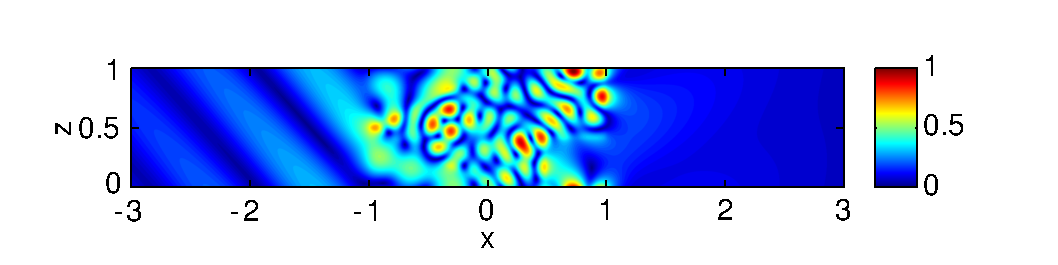
\includegraphics{gfx/eigenfunction.pdf}}\\\pause

\hfill Largest problem with our approach: $n\approx 10^7$.
\end{frame}

%\begin{frame}
%
%Waveguide model in \mycite{Tausch, Butler '02}  ($n=1000$)\\
%Convergence diagram:
%\scalebox{0.7}{\includegraphics{conv_hist_gamma3.pdf}}
%\end{frame}
%\begin{frame}{Computation time reduction}
%Standard infinite Arnoldi method:~\\
%
%\begin{center}\scalebox{0.6}{\includegraphics{cpu_time_percent.pdf}}~\\
%\end{center}
%Tensor infinite Arnoldi method:~\\
%\begin{center}\scalebox{0.6}{\includegraphics{cpu_time_percent_tensor.pdf}}\end{center}
%$\Rightarrow$ Room for improvement: faster derivative computation 
%\end{frame}
%
\begin{frame}[plain]%{Simulations - TIAR and waveguide eigenvalue problem}
Convergence and complexity: 
\scalebox{0.55}{\includegraphics{gfx/error_hist_wg.pdf}}\pause%
\scalebox{0.55}{\includegraphics[decodearray={0.2 0.3 1 0 1 0.8}]{gfx/complexity_comparison_bw.pdf}}
\end{frame}
\begin{frame}[plain]
 \begin{center}
   \resizebox{12cm}{!} {
    \begin{tabular}{c|c|c|c|c|c|c|}
     \cline{4-7}
		\multicolumn{3}{c}{}		&	 \multicolumn{2}{|c|}{CPU time } 			&	\multicolumn{2}{|c|}{storage of $Q_m$} 		\\
\hline
\multicolumn{1}{|c|}{$n$}		&	$n_x$	&	$n_z$	&	  IAR				&				WTIAR&	 		IAR 		&	 TIAR				\\
\hline
\multicolumn{1}{|c|}{462}		&	20	&	21	& 	 8.35 secs			&		2.58 secs		&		35.24 MB	&	7.98 MB				\\
\hline
\multicolumn{1}{|c|}{1,722}		&	40	&	41	& 	 28.90 secs			&		2.83 secs		&		131.38 MB	&	8.94 MB				\\
\hline
\multicolumn{1}{|c|}{6,642}		&	80	&	81	& 	1 min and 59 secs		&		4.81 secs		&		506.74 MB	&	12.70 MB			\\
\hline
\multicolumn{1}{|c|}{26,082}		&	160	&	161	& 	8 mins and 13.37 secs		&		13.9 secs		&		1.94 GB		&	27.52 MB			\\
\hline
\multicolumn{1}{|c|}{103,362}		&	320	&	321	& 	out of memory			&		45.50 secs		&		out of memory	&	86.48 MB			\\
\hline
\multicolumn{1}{|c|}{411,522}		&	640	&	641	& 	out of memory			&		3 mins and 30.29 secs	&		out of memory	&	321.60 MB			\\
\hline
\multicolumn{1}{|c|}{1,642,242}		&	1280	&	1281	& 	out of memory			&		15 mins and 20.61 secs	&		out of memory	&	1.23 GB				\\
\hline
\end{tabular}
}
 \end{center}
% \caption{CPU time and estimated memory required to perform $m=100$ iterations of IAR and WTIAR. The memory requirements
%for the storage of the basis is the same TIAR and WTIAR.}
 %\label{tbl:cputime_and_memory_IARvsTIAR}
{\small 
Using different computer: 
$n=9,009,002$, several hours CPU-time.}\pause
\begin{center}
\begin{minipage}{0.6\textwidth}
{\bf IAR:}\\
\scalebox{0.55}{\includegraphics{gfx/IAR_complexity2.pdf}}
\end{minipage}%
\begin{minipage}{0.6\textwidth}
{\bf TIAR+WEP:}
\scalebox{0.55}{\includegraphics{gfx/TIAR_complexity3.pdf}}
\end{minipage}
\end{center}
%figure with profiling aspects

\end{frame}
\section{Conclusions}
\begin{frame}
\begin{block}{New contributions}
  \begin{itemize}
    \item A structured discretization of a waveguide eigenvalue problem (WEP)
    \item A new algorithm: TIAR
    \item Specialization of TIAR to WEP
  \end{itemize}
\end{block}\pause
Key ingredients: WEP derivation
\begin{itemize}
  \item Floquet-Bloch leads to PDE QEP on strip
  \item Dirichlet-to-Neumann (DtN) map leads to PDE NEP 
  \item FEM with particular ordering of elements
\end{itemize}
Key ingredients: TIAR
\begin{itemize}
  \item Compact tensor-representation equivalent to IAR
\end{itemize}
Key ingredients: combination TIAR WEP
\begin{itemize}
  \item Handle singularities with Cayley transformation
  \item To compute $y_0$: FFT, Gegebauer polynomials, saddle-point structure, Schur complement
\end{itemize}
\end{frame}
\begin{frame}
\begin{center}
\Large
\bf Thanks for your attention!\\\vspace{0.5cm}
%\bf Thanks to COMSOL and KTH for DqF-financing!
%\vspace{2cm}
\end{center}
\medskip
Online material:
\begin{itemize}
  \item Preprint: \\\url{http://arxiv.org/abs/1503.02096}
  \item Software: \url{http://www.math.kth.se/~gmele/waveguide}
\end{itemize}

\end{frame}
%
%\begin{frame}
%\end{frame}
%
%\begin{frame}
%%\begin{minipage}{1.1\textwidth}
%%\vspace{1.8cm}
%%\end{minipage}
%\end{frame}
%
\end{document}


